\documentclass[../../Aurora C# unofficial manual.tex]{subfiles}

\begin{document}
	\subsection{Missile engines integrated into missile design}
	Original post can be found
	\href{http://aurora2.pentarch.org/index.php?topic=8495.msg114126#msg114126}{here}.
	\\\\
	
	In VB6, you research missile engines first and then use that engine within a missile design. This can be tedious, especially if you are not sure exactly what engine size you need. Therefore, for C\# the missile engine design has been removed from the Create Research Project window and integrated directly into the Missile Design window.
	
	The best engine and fuel efficiency tech will automatically be used, so the player decides on the engine size and power boost. The engine design takes place behind the scenes and is confirmed when you design the missile. This means you can play around with the engine design and missile design at the same time. See first screenshot below
	
	If no engine is required, just tick the No Engine option. See second screenshot.
	\begin{figure}[H]
		\centering
		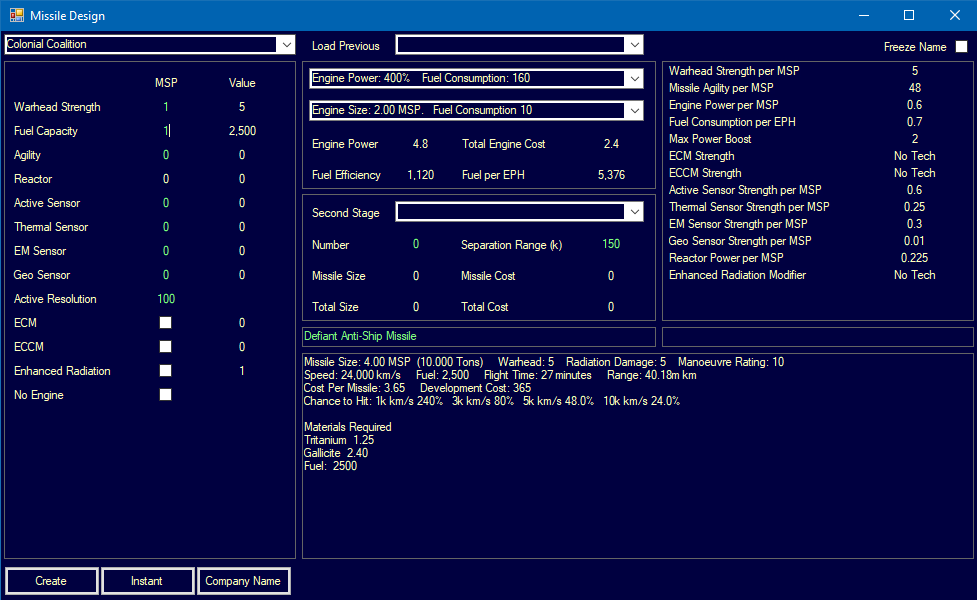
\includegraphics[width=0.7\linewidth]{images/MissileDesign}
		\caption[Missile Design]{Missile Design Example 1}
		\label{fig:missiledesign}
	\end{figure}
	\begin{figure}[H]
		\centering
		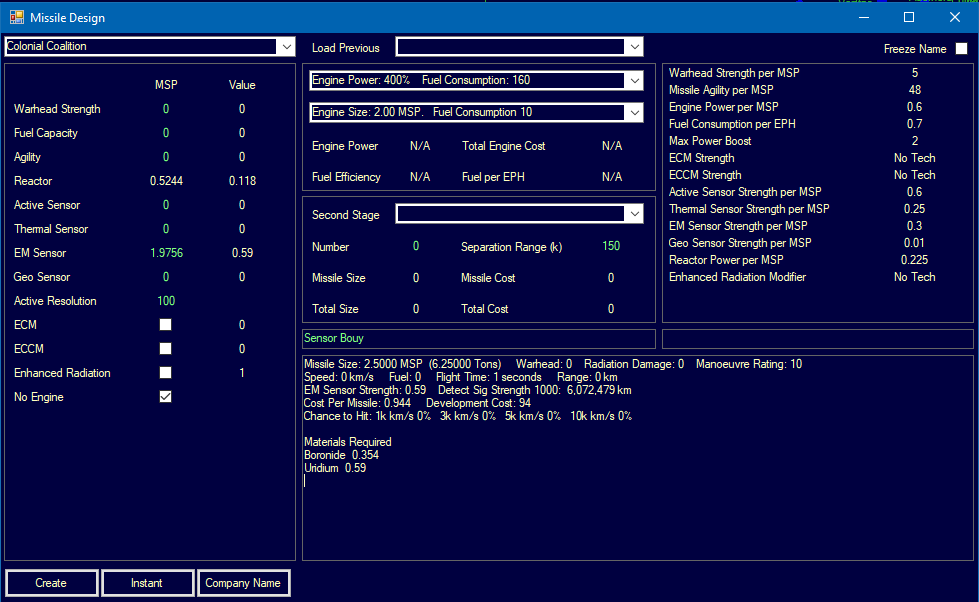
\includegraphics[width=0.7\linewidth]{images/MissileDesign2}
		\caption[Missile Design]{Missile Design Example 2}
		\label{fig:missiledesign2}
	\end{figure}
\end{document}